\section{Aprendizaje automático o \textit{Machine Learning}}
El aprendizaje automático es un método computacional que consiste en aprender a partir de los datos. 


\todo{Introducir Contexto histórico de ML, y su diferencia con el approach clásico de inteligencia artificial (dictado por reglas)} 



\begin{figure}[H]
    \centering
    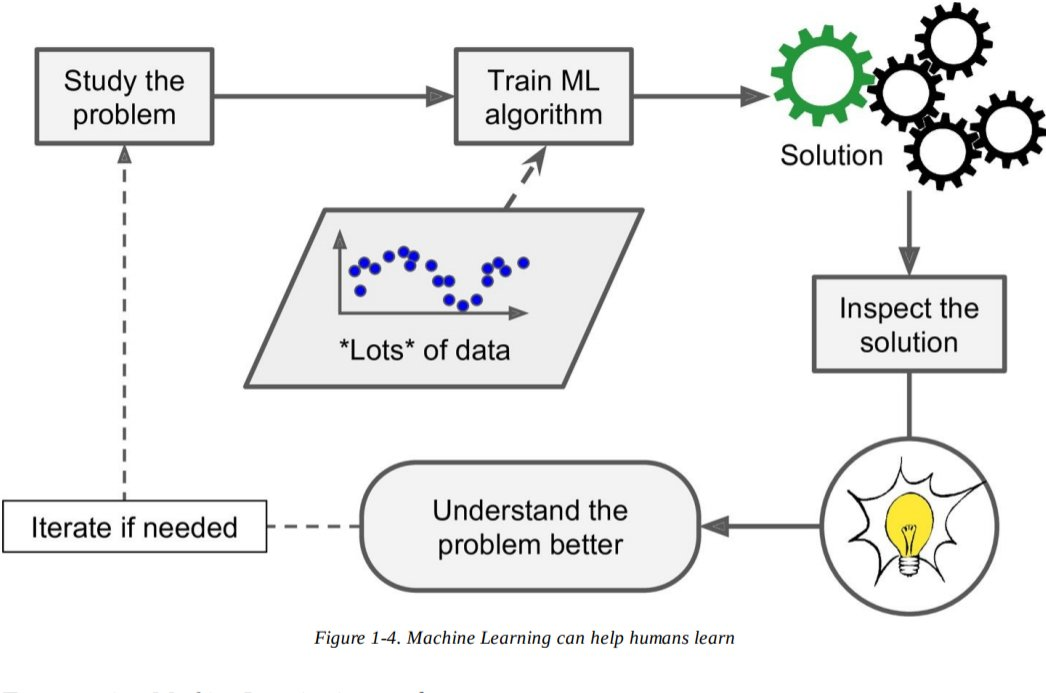
\includegraphics[scale=0.25]{documents/latex/figures/2/diagrama_ml.jpg}
    \caption{\todo{Diagramita tomado del Hands On with ML (Aurélien Géron). Podría poner algo similar}}
    \label{fig:ml_diagram}
\end{figure}


Existen diferentes formas de categorizar los algoritmos de aprendizaje automático. Nosotros nos vamos a centrar en la categorización de acuerdo a la cantidad de tipo de supervisión durante la fase de entrenamiento. Este aprendizaje puede ser:

\begin{itemize}
\item Supervisado, en donde se utilizan ejemplos previos que están "rotulados", es decir que posee una variable de respuesta conocida y se busca conseguir una predicción lo más certera posible sobre nuevos datos. \item No supervisado, donde el objetivo es encontrar distintos grupos o clusters dentro de los datos.
\item Semi-supervisado, en el que se trabaja con una combinación de datos etiquetados y no etiquetados y al aprendizaje por refuerzo
\item Por refuerzo, donde un \textit{agente} observa el entorno y realiza diferentes acciones para maximizar la recompensa. El modelo a aprender entonces es la estrategia que le permite tomar decisiones ante determinadas situaciones. 
\end{itemize}

En este trabajo nos vamos a centrar exclusivamente en tipo de aprendizaje supervisado.

\subsection{Aprendizaje supervisado}

Como mencionamos anteriormente, el aprendizaje supervisado trata de predecir una respuesta usando un modelo generado con datos correctamente etiquetados. Definido de manera formal, dado un set de datos $ \mathcal{D} = \{(x^n, y^n), n = 1...N\}$  buscamos aprender la relación entre el ejemplo $x$ y la variable de respuesta $y$ tal que al recibir un nuevo ejemplo $x^*$ la respuesta predicha $y^*$ sea precisa. Para definir de forma explícita a que nos referimos cuando hablamos precisión, es necesario construir una función $L(y^{pred}, y^{true})$.  

Podemos agrupar al aprendizaje supervisado en dos grandes categorías: la clasificación de nuevos datos, y la regresión, en donde el objetivo es la predicción de una variable continua. 

\subsection{Regresión logística}

\subsection{Support Vector Machines}

\subsection{Random Forest}

\subsubsection{Importancia de las variables}


\section{Pipeline del Modelo}

\section{Bases de datos genéticas}

\subsection{Humsavar}

Humsavar es una recopilación de SNPs anotados manualmente 


\section{Clinvar}







% En esta sección detallaremos cada unos de los datasets usados durante nuestro trabajo, las distintas fuentes de atributos, y el esquema de clasificación usado.

% \section{Análisis de los Datasets}

% \subsection{Dataset VarQ}

% El primer paso que tomamos fue realizar un análisis del dataset VarQ. Este dataset fue generado por la herramienta homónima generada en el BIA (Plataforma Bioinformática Argentina) por Leandro Radusky. Esta herramienta permite extraer datos estructurales de variantes proteicas de un sólo aminoácido (SAS, por sus siglas en inglés) tomando información de diferentes bases de datos o aplicaciones (PDB, PFam, 3DID, entre otras), permitiendo el análisis manual de los diferentes cambios estructurales, como el tipo de actividad, el plegamiento, si pertenece a un sitio activo, o si forma parte en interfaces proteína-proteína \cite{Radusky2017}. 

% \begin{figure}[H]
%     \centering
%     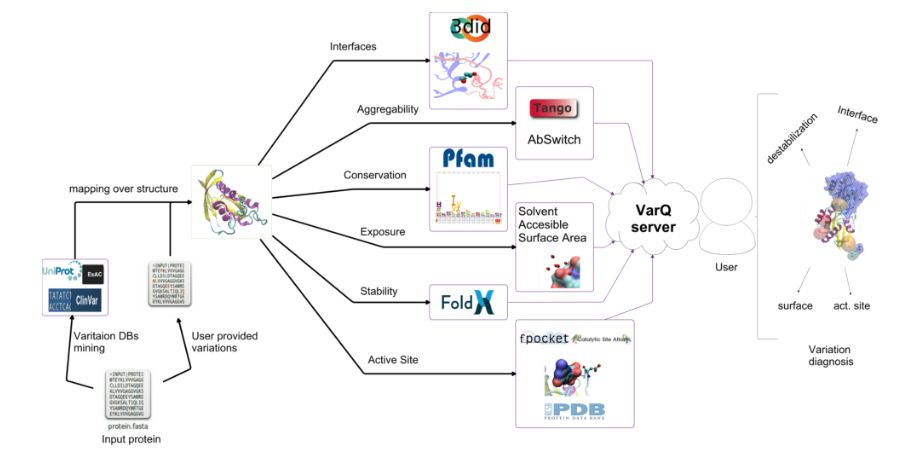
\includegraphics[scale=0.4]{documents/latex/figures/1/pipeline.png}
%     \caption{Pipeline de extracción de datos de la herramienta VarQ. Esta figura fue extraída de la tesis de doctorado de Leandro Radusky.}
%     \label{fig:varq_pipeline}
% \end{figure}


% Este dataset fue un acercamiento inicial al problema de predecir si a partir de una mutación en el gen. Para esto verificamos la calidad de cada una de las variables incluyendo el tipo. Validando el tipo de cada una de las variantes pudimos encontrar algunas de las que no se conoce a ciencia cierta su patogenicidad, por lo que fueron removidas. El dataset VarQ final tiene aproximadamente 17,8 mil variantes, de los cuales:

% \begin{itemize}
%     \item 11,7 mil están catalogados como benignos.
%     \item 6,1 mil están catalogados como patogénicos.
% \end{itemize}

% Posee 12 columnas o variables: 

% \begin{itemize}
%     \item Mutant: Código identificatorio de la variante, compuesto por el código Uniprot, la posición del aminoácido donde ocurre la variación, y el cambio de aminoácido.
%     \item SASA (Solvent-Accessible Surface Area): El área del aminoácido accesible por un solvente.
%     \item SASA Percentage: El porcentaje del SASA sobre la superficie del aminoácido.
%     \item B-FACTOR: Factor de temperatura correspondiente a un aminoácido en la proteína. Una mayor temperatura indica que el aminoácido pertenece a una zona potencialmente de mayor movilidad.
%     \item Switchability: Factor de \textit{switching} del aminoácido \cite{Diaz2014}. Genera cambios en el plegamiento y por ende en la función de la proteína. 
%     \item Aggregability: Usando el software Tango \cite{Fernandez-Escamilla2004}, evalúa la propensión del aminoácido a generar agregación desde un punto de vista estructural
    
% \end{itemize}

